\documentclass[tikz,border=10pt]{standalone}
\usepackage{tikz}
\usetikzlibrary{arrows.meta,positioning}

\tikzset{
  card/.style={draw=blue!70!black, line width=1.2pt, rounded corners=3pt, minimum width=4.8cm, minimum height=1.1cm, align=center, fill=none},
  result/.style={draw=orange!80!black, line width=1.2pt, rounded corners=3pt, minimum width=4.8cm, minimum height=1.1cm, align=center, fill=none},
  flow/.style={-{Stealth[length=3mm]}, line width=1.2pt, draw=black!70}
}

\begin{document}
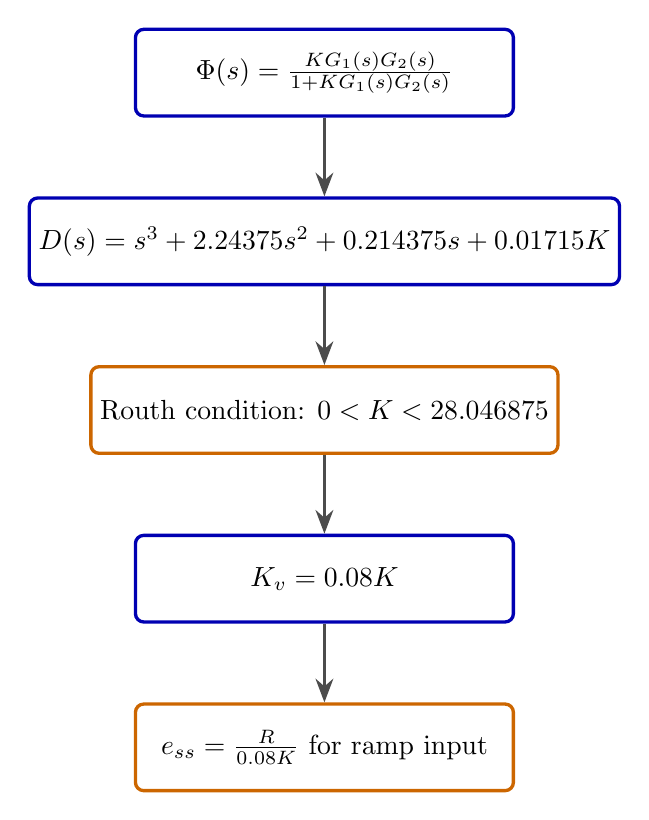
\begin{tikzpicture}[node distance=1.0cm]
  \node[card] (a) {$\Phi(s)=\frac{K G_1(s) G_2(s)}{1 + K G_1(s) G_2(s)}$};
  \node[card, below=of a] (b) {$D(s)=s^3 + 2.24375 s^2 + 0.214375 s + 0.01715 K$};
  \node[result, below=of b] (c) {Routh condition: $0 < K < 28.046875$};
  \node[card, below=of c] (d) {$K_v = 0.08 K$};
  \node[result, below=of d] (e) {$e_{ss} = \frac{R}{0.08 K}$ for ramp input};

  \draw[flow] (a) -- (b);
  \draw[flow] (b) -- (c);
  \draw[flow] (c) -- (d);
  \draw[flow] (d) -- (e);
\end{tikzpicture}
\end{document}
